\section{Planificació}

    \paragraph{}
    L'objectiu d'aquest apartat de la memòria és presentar les diferents planificacions que s'han portat a terme per encarar el projecte en cada una de les convocatòries matriculades.

    \subsection{Planificació Febrer del 2014 -\ Juliol 2014}

        \paragraph{}
        Aquest projecte va ser matriculat per primera vegada al Febrer del 2014 amb la intenció de presentar-lo com a principis de juliol del mateix any. La idea inicial era aprofitar el mes de gener per avançar feina i disposar així d’un total de sis mesos per realitzar el projecte.

        Al març del 2014 vaig començar a treballar a jornada completa i el projecte va deixar d’avançar a la velocitat esperada. Es van començar a patir forts endarreriments sobre la planificació original fins al punt que el projecte va quedar completament aturat. La figura~\ref{fig:firstPlan} mostra en línies generals la planificació que s’hagués volgut portar a terme en cas de normalitat i ressaltat en vermell la part que es va veure interrompuda.

        \begin{figure}[h]
                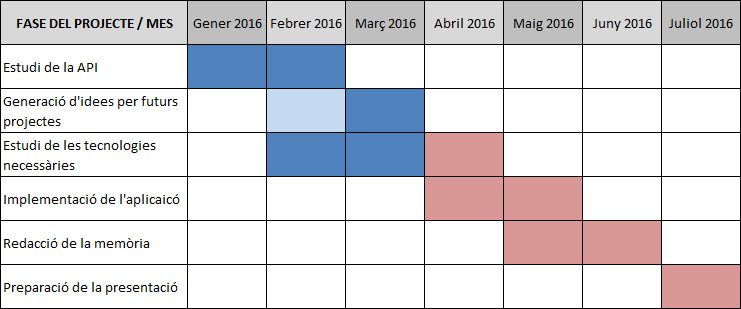
\includegraphics[width=\linewidth]{01/firstPlan}
                \centering
                \caption{Planificació original \emph{Febrer 2014 -\ Juliol 2014}.\label{fig:firstPlan}}
        \end{figure}

        La falta de temps per realitzar un projecte acceptable, conjuntament, a la poca capacitat de maniobra de les que es va disposar entre els mesos de Març i Juliol, va provocar que es descartés la possibilitat de presentar el projecte durant la convocatòria prevista inicialment.

    \subsection{Planificació Febrer del 2016 -\ Setembre 2016}

        \paragraph{}
        A  conseqüència de l’extinció del pla d’enginyeries 2003, el projecte es torna a matricular al Febrer del 2016, tenint en consideració que s'hauria de començar pràcticament de 0.

        Donada la diferència de temps entre la primera inscripció i la segona, l’\gls{API} de FamilySearch s'havia vist sotmesa a grans canvis i la major part del material estudiat i coneixements tècnics adquirits fa dos anys, quedaven completament antiquats.

        A pesar de matricular el projecte a mitjans de Febrer es coneixia que aquest no podria ser començat amb agilitat fins a principis d’abril a causa d'una situació excepcional en l'àmbit laboral. Gràcies a la disponibilitat d’una pròrroga extraordinària, que permetia estendre el període d'entrega fins a finals de setembre, la finestra de temps disponible per completar el projecte rondava els cinc o sis mesos.

        Cal tenir en compte que la disponibilitat horària en el dia a dia de cara a treballar en el projecte era molt reduïda i en conseqüència, realitzar una bona planificació era essencial si es volien evitar els mateixos problemes que van provocar l’abandonament del projecte en el seu primer intent.

        Tant en la figura~\ref{fig:actualPlan}, com en les seccions que segueixen a continuació, expliquem com va ser planificada i executada la feina entre els mesos d'abril i setembre.

        \begin{figure}
            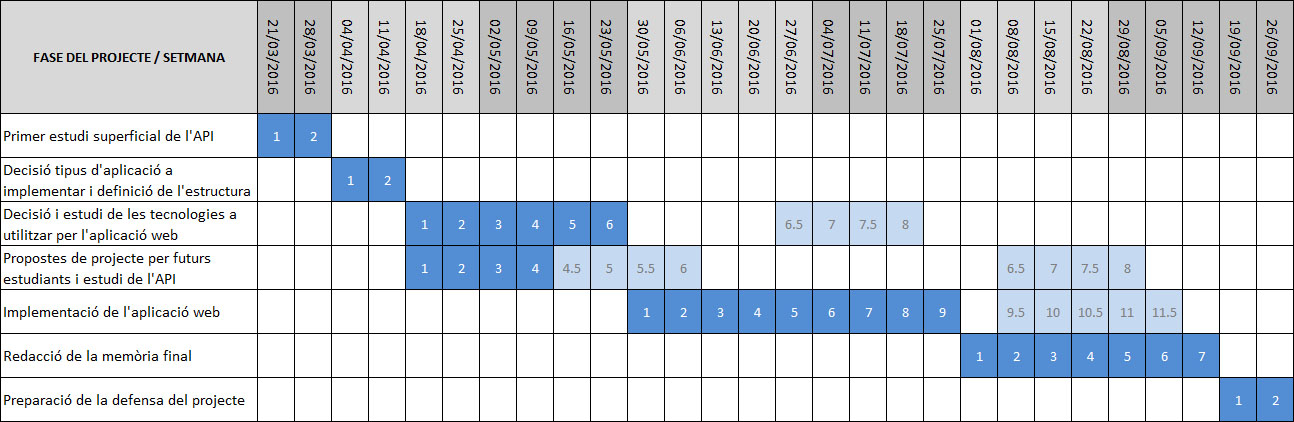
\includegraphics[scale=0.5, angle=90]{01/actualPlan}
            \centering
            \caption{Planificació final \emph{Febrer 2016 -\ Setembre 2016}.\label{fig:actualPlan}}
        \end{figure}

        \subsubsection{Segona quinzena de Març}

            \paragraph{}
            En aquest petit període de temps es va realitzar el primer estudi superficial sobre l'\gls{API} de FamilySearch amb la finalitat d’observar quins canvis s'havien produït durant els darrers dos anys i com aquests podien afectar o modificar la proposta inicial inscrita del projecte.

            L'objectiu d'aquesta repassada ràpida era la de proporcionar una visió global sobre certes limitacions que podrien afectar el desenvolupament del projecte i ens permetés elaborar una planificació coherent de com afrontar i estructurar la feina a realitzar.

        \subsubsection{Primera quinzena d'Abril}

            \paragraph{}
            Tot i que l’estudi sobre la informació disponible a través de l'\gls{API} es trobava en els seus inicis es va aprofitar aquesta quinzena per decidir quina mena d’aplicació volíem implementar. Aquesta decisió obriria pas a la recerca i estudi sobre quines tecnologies serien més adients de cara a la implementació dels exemples i les comunicacions amb l'\gls{API} de FamilySearch.

            També s'aprofitaria aquesta quinzena per familiaritzant-nos amb la diferent documentació disponible sobre l'\gls{API} de FamilySearch i plantejar-ne l’ordre d'estudi.

        \subsubsection{Segona quinzena d'Abril -\ Finals de Maig}

            \paragraph{}
            Aquest període inicial del projecte resultava crucial de cara a incorporar les eines necessàries al nostre coneixement que ens permetrien completar un dels objectius principals del projecte durant els mesos següents.

            Així doncs, l'objectiu era el de detallar i estudiar tots els aspectes referents a la part tècnica de l’aplicació. Escollir de forma correcta era indispensable si volíem evitar tancar-nos portes abans de començar o assegurar-nos de què utilitzàvem eines eficients que oferien un bon balanç entre esforç i qualitat.  Els punts coberts durant aquesta fase van ser:

            \begin{itemize}
                \item Esbrinar els components principals que conformen una pàgina web avui en dia i com interactuen.
                \item Conèixer les diferents tecnologies disponibles per cada un d’aquests components.
                \item Escollir del grup de tecnologies estudiat les més adients per fer front als objectius del projecte i estudiar-les a fons.
            \end{itemize}

            \paragraph{}
            El segon objectiu d’aquesta fase consistia en estudiar a fons l'\gls{API} de FamilySearch per obtenir una idea més concreta quina mena de projectes es podrien arribar a realitzar i quins no. Aquest exercici ens ajudaria a comprendre quins exemples tindria més sentit implementar per tal de demostrar la potencialitat i abast de l'\gls{API}.

        \subsubsection{Mesos de juny i juliol}

            \paragraph{}
            Gairebé tot l’esforç durant aquests dos mesos es concentraria en la implementació de l’aplicació web. Es va decidir prioritzar aquesta tasca per sobre de la generació d'idees i l'estudi final de l'\gls{API} per dos motius.

            Gairebé tot l’esforç durant aquests dos mesos es concentraria en la implementació de l’aplicació web. Es va decidir prioritzar aquesta tasca per sobre de la generació d'idees i l'estudi final de l'\gls{API} per dos motius.

            A pesar dels avantatges que oferia desenvolupar l'aplicació en primer lloc, com a contrapartida, també significava tirar endavant una part important del projecte amb el risc de no haver arribat a conèixer la totalitat de l'abast de l'\gls{API}.

        \subsubsection{Mes d'agost}

            \paragraph{}
            L'objectiu del mes d'agost era fer front a tota aquella part del projecte que havia quedat oblidada fins aquest moment. En concret:

            \begin{itemize}
                \item Redactar la memòria del projecte.
                \item Detallar les diferents propostes de projecte pels futurs estudiants.
                \item Implementar algunes parts dels continguts estàtics de l'aplicació web.
            \end{itemize}

        \subsubsection{Mes de setembre}

            \paragraph{}
            El mes de setembre s'utilitzaria com a marge de maniobra per acabar de tancar aquelles tasques del projecte que poguessin estar sotmeses a petits retards. Segurament, l'acabat de redacció de la memòria i petits retocs en l'aplicació web.

            També s'aprofitaria la part final del més, un cop el projecte estigués entregat, per preparar la defensa.
